\section{Depth-Based Tiebreaking for A*}

\label{sec:depth}

As shown in the previous section, the search spaces of Zerocost domains have many zero-cost edges,
resulting in a large final plateau ($\plateau{f^*,0}$). In a final plateau,
all nodes have $h=0$, so $h$-based tiebreaking cannot provide
useful guidance toward a goal. Thus, we need a new metric for discriminating among nodes
in the plateau so that the search algorithm can make progress in the plateau.

We define the \emph{depth} of a node as an 
integer representing the distance (number of steps) from the
\emph{entrance} of the plateau.  An \emph{entrance} of the plateau is
the first node which encountered in the plateau, along the path from the
initial node. These notions are depicted in
\refig{fig:plateau-depiction} (subfigure 1). 
Another way to think about depth is consider the problem of finding an exit from a particular plateau (i.e., finding either a goal node or exhausting the plateau) a unit-cost search space by itself -- the depth is analogous to a $g$-value for this space.
%It is equivalent to the $g$-value which is
%restricted to a particular plateau and is assuming the unit cost edges.

\begin{figure}[htbp]
  \centering
  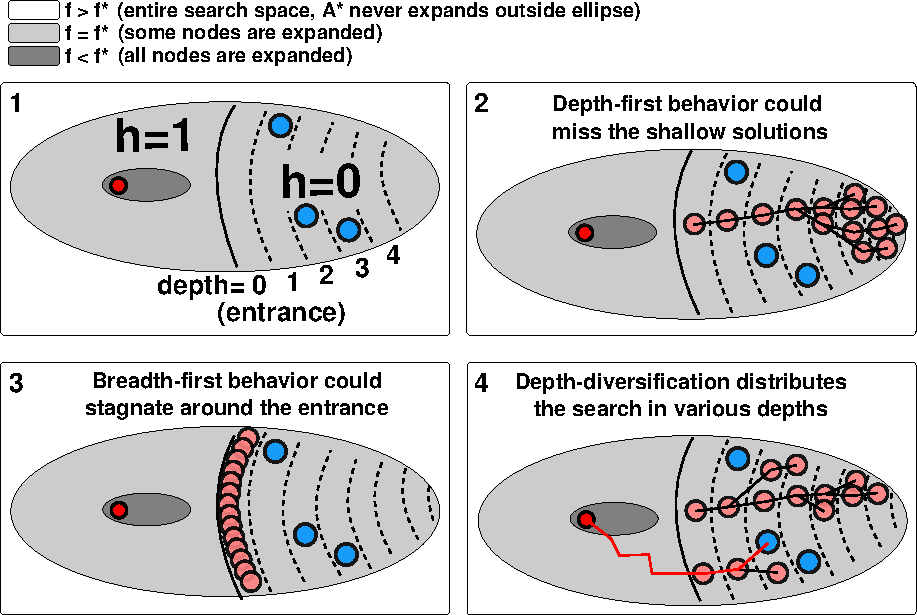
\includegraphics{img/astar/plateau-2.pdf}
 \caption{(\textbf{Subfigure 1}) The nodes in a plateau are divided into several layers, and each layer have the corresponding depth. Since all nodes have $f=f^*$, depth does not affect optimality. The goals in both shallower or deeper region yield cost-optimal solutions.
 (\textbf{Subfigure 2}) \lifo tiebreaking strategy results in depth-first behavior in a
 plateau, which could miss solutions if they are concentrated near the entrance.
 (\textbf{Subfigure 3}) \fifo tiebreaking strategy results in  breadth-first behavior in a
 plateau, which could fail to reach a solutions in deeper layers within the time limit.
 (\textbf{Subfigure 4}) Depth-based diversification allows \astar to search the plateau space
 sparsely in a less biased, more uniformly and manner. This balances exploration and exploitation, avoiding the problems with both \lifo (depth-first) and \fifo (breadth-first) behavior.
 }
 \label{fig:plateau-depiction}
\end{figure}

The depth $d(n)$ of a
node $n$ is 0 when $n$ and the parent node $m$ have different key
values for a sorting strategy, and $d(n)=d(m)+1$ when they have the same
key values: For example, in \astar with $h$-based tiebreaking, the key
values of a node are represented as a vector $[f,h]$, and they are same
when they are pairwise equivalent (i.e. $f(n) = f(m) \land h(n) =
h(m)$).  Having the same key values means that $n$ and $m$ are in the
same plateau.

The traditional \lifo and \fifo tiebreaking strategy 
search the plateau region in decreasing and increasing order of the depth, respectively.
The \lifo strategy always selects the most recently generated node
within $\plateau{f,h}$, and the behavior in the plateau is equivalent to depth-first search.
Thus, \lifo always selects the largest depth
buckets, as depicted in \refig{fig:plateau-depiction} (subfigure 2).
Similarly, the behavior of the \fifo strategy 
in a plateau is equivalent to breadth-first search. Thus \fifo 
always selects the nodes with least depth (subfigure 3).
Note that  $[f,h,\lifo]$ is equivalent to $[f,h,-d,\lifo]$ and
$[f,h,\fifo]$ is equivalent to $[f,h,d,\fifo]$.

The problem with these traditional strategies is that we have no knowledge
regarding whether the goals are located close to or far from the entrance. Recall
that since $f=f^*$, all goal nodes in the final plateau are optimal with respect to solution cost.
regardless of the depth.%: A goal node in a shallower region or a deeper region both yields a cost-optimal solution. 
However, until we find a
solution, we do not know how the goals are distributed among various
depths. In some problem instance the goals can be concentrated around
the entrance, and in other problem instances the goals can be
concentrated at some large depth. % $k$.  k never used below?

In the former case, (\fifo), whose breadth-first behavior naturally
focuses the search around the entrance favoring the smaller depths,
should perform well, but in the latter case, exhaustively searching
the shallower depths can result in not finding any solutions within
the time limit because \fifo may never reach the depth where the goals
exist.  On the other hand, \lifo behaves in a depth-fist manner, so it
may reach solutions at deeper depths quickly, but risks missing
solutions at shallower depths.  Thus, both \fifo and \lifo tiebreaking
are prone to failures due to pathological cases.

In order to avoid focusing the search at the wrong depths (too shallow/deep), 
the safest policy seems to be to simply \emph{diversify} the depths which are being searched,
in order to avoid any depth-based biases which could lead to pathological behavior.
In our proposed \emph{depth diversification} strategy, the nodes are inserted into buckets
associated with depths, and upon expansion, search effort is distributed in a more balanced manner
among various depths (\refsec{sec:theoretical-characteristics} defines ``more balanced''  more precisely).
Nodes are not  ``sorted''
according to increasing or decreasing order of depth -- instead we try to 
``diversify'' the node expansion within the plateau.
We denote this depth diversification criterion as $\depth$. 
For example, $[f,h,\depth]$ first breaks ties according to $h$ values,
then uses the $\depth$ criterion to break ties in $\plateau{f,h}$.
%We denote such a diversification family of
%tiebreaking strategies by enclosing it in brackets such as $[f,h,\depth]$.

In order to diversify the expansion among depths, we simply
iterate over the depth buckets. An index $d_c$,
 which stores the depth (bucket index)  which was selected in the last expansion,
is initialized to 0.
At each expansion, the counter is decremented ($d_c\leftarrow d_c-1$) and
a node from  bucket $d_c$ is expanded. When $d_c$ reaches below 0, then $d_c$
is reset to the current largest depth in the plateau.

In an earlier, conference paper, we used a nondeterministic,
randomized implementation of this idea \cite{Asai16}, but we use a deterministic
implementation here because it eliminates the possibility of results being influenced by random seeds,
and also facilitates the  theoretical analysis below in \refsec{sec:theoretical-characteristics}.

% We later show that
% \fifo and \lifo strategies are incomplete when the size of the plateau
% region is inifinite, while our \id is probabilistically complete.

\subsection{The Scope Captured by Depth-Based Tiebreaking}

Depth-based tiebreaking has no effect when the key values for measuring
the depth are always updated and thus all nodes have depth 0. A key
value is a single $f$ when $h$-based tiebreaking is not present, and a
pair of $f$ and $h$ when $h$-based tiebreaking is present. When all
nodes have depth 0, the search is equivalent to the case where 
the depth-based strategy is not present.\todo{mentioning ``keys'' seems unnecessarily complicated, and  ```key'' doesn't seem to be used much in the rest of the paper -- simpler+sufficient to just say that 
``depth diversification has no effect when there are no plateaus after the higher priority tiebreaking criteria (e.g., in a [f,h,<d>] strategy, when there are no [f,h] plateaus), which occurs when the problem only has positive cost operators'' ?}
% 
This happens when the target problem only has 
operators with positive cost. %\footnote{not to be confused with non-negative cost.  XXXshouldn't be necessary, positive doesn't include 0 for any standard def} 
Let a node $n$ is reached from a node $m$. \todo{is this par necessary?}
Assume
 $g(n)>g(m)+c$ where $c$ is a positive edge cost, and the parent of $n$
 is updated to $m$.

\begin{itemize}
 \item 
       If $f(n)=f(m)$, $h(n)<h(m)$ should hold because the new value of
       $g(n)$ is $g(m)+c>g(m)$. Therefore the depth is 0.
 \item If $h$-value is unchanged and $g$ is increased due to a positive
       cost edge, then $f$ is also increased, thus the depth is 0.
\end{itemize}

One might wonder what if the evaluated (?) nodes (?) are already visited (?) from
another parent (old (?)parent) with smaller $g$ value, and the new $g$ value does not change it (?),
which may cause the new parent and the child node may have the same $f$ and
same $h$. It does not result in a positive depth because it does not update the parent. The depth of a
child remains the old value (using the old parent), which is 0.\todo{rewrite par -- terminology is inconsistent and pronouns are ambiguous}


\subsection{Tiebreaking within Depth Buckets}

Consider a tiebreaking strategy such as $[f,h,\depth]$ which applies a depth-diversification tiebreaking.
After the $\depth$ criterion is applied, 
there may be multiple nodes within the same depth bucket, so a
default tiebreaking criterion is still necessary to break ties among them.
We can, for example, apply \lifo, \fifo or \ro (random order) policies
at this level.

There could be still a room for heuristic-agnostic improvements at
this level, \todo{what is ``this level'': same level as $\depth$ (in which case these 2 pars don't seem to fit in this subsection), or after depth?} while this is not in the scope of this paper.
For example, while depth metric measures and diversifies the depth in a plateau,
other techniques can non-trivially diversify the search in a breadth direction.
Such techniques may include pruning techniques such as 
Symmetry Breaking \cite{Fox1998,pochter2011exploiting,domshlak2013symmetry}
or Partial Order Reduction \cite{hall2013faster,wehrle2013relative}.

While these methods are most often described as ``pruning techniques'',
it can be rephrased as ``removing the cardinality bias to particular set
of nodes which share the same characteristics'' because they both aim to
prune the redundant nodes. Note that redundancy causes a biased 
search effort. For example, imagine we have a
set of nodes $S=\{a_1, a_2, a_3, a_4, b, c, d\}$ where
$A=\{a_1, a_2, a_3, a_4\}$ are ``redundant'' in some measure (e.g. by Symmetry,
Partial-Order). 
If a search algorithm expands $S$ by random selection, it favors the
group $A$ by giving a 4 times larger chance of expansion than $b$,
$c$ or $d$.

% \todo{compare id,fifo and id,lifo}
CommentOnTheDeletedActionOrderingText\todo{Although there's no need to show new results for action ordering, 
it may be a good idea to summarize+point to the AAAI16 action ordering experiment, in order to eliminate concerns that
all our results are somehow specific to one particular action order.}
% However we use a Random Order (\ro) criterion, which 
% randomly selects an element from the depth bucket selected by the depth-based tiebreaking.
% This is because the effectiveness of the tiebreaking behavior within a bucket
% can be affected by accidental biases, e.g., names/orders of action schema in the PDDL domain
% definition \cite{vallati2015effective}.
% %Finding the best action ordering is not the scope of this paper.
% Thus, we avoid bias at this level of tiebreaking by using \ro and assess its expected/average
% performance.

% Among \fifo, \lifo and \ro, the natural criterion is Random Order.
% This is because the effectiveness of the third-level tiebreaking behavior
% is affected by the accidental bias in action ordering in the PDDL domain
% definition.  Recent work \cite{vallati2015effective} showed that the
% planner performance is greatly affected by changing and tuning the action ordering
% (and also variable ordering, but it is irrelevant to the tiebreaking behavior). 
% However, finding the best third-level tiebreaking is not the scope of this paper.
% Thus, focusing on \ro and assess its expected/average
% performance is the most reasonable practice to understand the behavior of second-level,
% depth-based tiebreaking.

\subsection{Theoretical Characteristics of the Depth Distribution}
\label{sec:theoretical-characteristics}

We give further insight into the search behavior of our implementation
of depth-based diversification.
As described above, our implementation performs a deterministic, round-robin samping from the available depth buckets.
%iterates from the largest depth to 0.

%We are particularly interested in how the expansions happen among the
%various depths in the plateau region.
We are particularly interested in how the nodes selected for expansion are distributed 
among the various depths in a plateau region.
Using a simplified model where the plateau region is a tWe show that the probability of expanding a node in a particular depth
can be represented by a simple formula.  Although the notion of
probability does not fit well with deterministic \fifo or \lifo
default tiebreaking, it is meaningful in the case of \ro (random
order) default tiebreaking.

%% danger!!
% \begin{theo}[Uniformness of the search]
%  Assume the search space forms a tree of fixed width $w\geq 2$.
%  After enough number of iterations $D$,
%  the chance of expanding each node is unaffected by the depth of the
%  node, if the depth $d$ is small relative to $D$.
% \end{theo}

% I no longer claim the distribution is uniform.
As a preparation, we first show that the number of expansion happened to each depth decreases
linearly to the depth.
% 
Assume that each depth bucket never exhausts as a result of
expansion.  If the expansion of a node in the largest depth $D\geq 0$ resulted
in more nodes in the same plateau, then the newly generated nodes have
depth $D+1$.  Also, as we explained in the previous section, the
expansion is diversified by a sequence of iterations from the current
largest depth to 0.  It means that when the current maximum depth of
the plateau is $D\geq 0$, the number of iteration happened so far is also $D$.\todo{what if all the nodes generated in an iteration, all nodes were previously generated? In this case numiterations < D. Does the assumption regarding the plateau need to be changed to: plateau such that every node has w>=2 children which were not previously generated?}
Therefore, at the end of the $D$'th iteration, each depth $d$ has
been expanded exactly $D-d$ times, meaning that the chance of
expanding each depth is decreasing as the depth increase.

% However, it does not mean that this strategy favors the nodes in the
% shallower region.
% This is because the number of nodes in each depth is
% exponential to $d$, which is common in practice (we verify this in the
% later experiments).
Now we show the formula which represents the probability of expanding a node in a particular depth.
We assume that the plateau region form a tree of a fixed branching factor
$w\geq 2$, rather than a graph with indefinite number of successor
nodes.  Under this assumption, each expansion of depth $d$ results in
$w$ new nodes in depth $d+1$. Also, if there are initially
$D$ nodes in depth 0, each depth bucket never exhausts until the end of $D$'th
iteration (when depth 0 becomes empty).

% $D-d$th expansion in the $D$th iteration expands the depth $d$.
At the end of $D$th iteration,
each depth $d-1$ is expanded $D-(d-1)$ times in the preceding $D$ iterations.
Therefore, the total number of nodes that have been in depth $d$, including those
that have been expanded so far, is $w(D-d+1)$.
Expansion has happened $D(D-1)$ times in total, and depth $d$ is expanded $D-d$ times.
Thus, the probability of expanding each node in depth $d$ is
$\frac{D-d}{D(D-1)\cdot w(D-d+1)}=\frac{1}{wD(D-1)}(1-\frac{1}{D-d+1})$.  \qed

Notice that $\frac{1}{D-d+1}$ is negligible if $D \gg d$.
Thus, after enough number of iterations (large $D$), the nodes are 
expanded in an approximately equal probability $\frac{1}{wD(D-1)}$ in the shallower region, and is
unaffected by the depth of the node.
However, the nodes near the largest depth has less probability, showing
some balance in exploration and exploitation.

The important point of this characteristics is that this distribution is maintained at any point of the search
until the solution is found. In fact, any depth-selection criterion, including the least depth selection (\fifo) or
the largest depth selection (\lifo), result in the same distribution if all nodes are to be expanded (each depth
$d$ is expanded $Dw^d$ times), but their online characteristics are not.
%
\todo*{maybe \lifo and \fifo should be analyzed wrto this tree model and compared directly to each other as well as
$\depth$?}
\todo*{less priority -- lets add it when required by the reviewers. unused texts are in unused/lifo-fifo-distribution.tex}
